%%%%%%%%%%%%%%%%%%%%%%%%%%%%%%%%%%%%%%%%%
% University of Milano Bicocca
% Created by Davide Costantini, Gianlorenzo Martini, Khalil Mohamed Khalil, Lorenzo Occhipinti, Luca Milazzo
%%%%%%%%%%%%%%%%%%%%%%%%%%%%%%%%%%%%%%%%%

%----------------------------------------------------------------------------------------
%	PACKAGES AND DOCUMENT CONFIGURATIONS
%----------------------------------------------------------------------------------------

\documentclass[12pt]{article} 

\usepackage[left=3cm, right=3cm]{geometry} % insert here document layout options
\usepackage{natbib} % Required to change bibliography style to APA 
\usepackage{tabularx,booktabs,tabulary,array,graphicx,url}
\usepackage{graphicx,wrapfig,lipsum}
\graphicspath{ {./images/} }
\usepackage[table,xcdraw]{xcolor}
\usepackage{multirow}
\usepackage{caption}
\usepackage[export]{adjustbox}
\usepackage{float}
\usepackage{indentfirst} 
\usepackage{subfig}
\usepackage{listings}
\renewcommand{\figurename}{Fig.}
\usepackage{adjustbox}
\usepackage{pifont}
\usepackage{listings}
\usepackage{color}
\definecolor{dkgreen}{rgb}{0,0.6,0}
\definecolor{gray}{rgb}{0.5,0.5,0.5}
\definecolor{mauve}{rgb}{0.58,0,0.82}

\lstset{frame=tb,
  language=Java,
  aboveskip=3mm,
  belowskip=3mm,
  showstringspaces=false,
  columns=flexible,
  basicstyle={\small\ttfamily},
  numbers=none,
  numberstyle=\tiny\color{gray},
  keywordstyle=\color{blue},
  commentstyle=\color{dkgreen},
  stringstyle=\color{mauve},
  breaklines=true,
  breakatwhitespace=true,
  tabsize=3
}
\usepackage{hyperref} % \usepackage[hidelinks]{hyperref} use the 'hidelinks' option to remove red boxes from links
\newcommand*\rot{\rotatebox{90}} % custom command to rotate columns/rows names in tables


%\usepackage{times} % Uncomment to use the Times New Roman font

%----------------------------------------------------------------------------------------
%	DOCUMENT INFORMATION
%----------------------------------------------------------------------------------------

\title{ Progetto Questionari 1 - Ingegneria del Software  UNIMIB 2021/2022} % Title

\author{Davide Costantini, Gianlorenzo Martini, Khalil Mohamed Khalil, \\ Lorenzo Occhipinti, Luca Milazzo} % Author name

\date{30/01/2022} % Date for the report

\begin{document}

\maketitle % Insert the title, author and date
\newpage
\tableofcontents \newpage
\section{Visione}
\subsection{Introduzione}
Prevediamo la realizzazione di un'applicazione web chiamata UNIMIB Questionari, un ambiente all'interno del quale gestire e compilare i questionari, dotata di alta usabilità, tolleranza ai guasti, sicurezza e performance.
\subsection{Posizionamento}
\subsubsection{Forumlazione del problema}
I prodotti già esistenti che propongono servizi di questo tipo spesso mancano della componente comunitaria. Per esempio, non sempre è possibile costruire un questionario a partire dalle domande di altri utenti o creare una vera e propria bacheca pubblica per i questionari stessi.
\subsubsection{Parti interessate}
I destinatari del sistema possono appartenere ad una qualsiasi categoria di utente che sia in grado di navigare nel web e questo definisce un ampio spettro di copertura.

\section{Analisi e progettazione}
\subsection{Glossario}

\begin{table}[H]
\begin{adjustbox}{max width=1.1\textwidth,center}
\begingroup
\setlength{\tabcolsep}{10pt} 
\renewcommand{\arraystretch}{2}
\begin{tabular}{llll}
\multicolumn{3}{c}{\textbf{Glossario}}                                                                                                                                                                                                                                                                                                                                     \\ \hline
\rowcolor[HTML]{3531FF} 
\multicolumn{1}{|l|}{\cellcolor[HTML]{3531FF}{\color[HTML]{FFFFFF} \textbf{ID}}} & \multicolumn{1}{l|}{\cellcolor[HTML]{3531FF}{\color[HTML]{FFFFFF} \textbf{Termine}}} & \multicolumn{1}{l|}{\cellcolor[HTML]{3531FF}{\color[HTML]{FFFFFF} \textbf{Definizione}}}                                                                                                         \\ \hline
\multicolumn{1}{|l|}{1}                                                          & \multicolumn{1}{l|}{Utente}                                                          & \multicolumn{1}{l|}{Un qualsiasi utente che utilizza il sistema.}                                                                                                                                \\ \hline
\multicolumn{1}{|l|}{2}                                                          & \multicolumn{1}{l|}{Utente registrato}                                               & \multicolumn{1}{l|}{Un utente che possiede un account.}                                                                                                                                          \\ \hline
\multicolumn{1}{|l|}{3}                                                          & \multicolumn{1}{l|}{Utente non registrato}                                           & \multicolumn{1}{l|}{Un utente che non possiede un account.}                                                                                                                                      \\ \hline
\multicolumn{1}{|l|}{4}                                                          & \multicolumn{1}{l|}{Servizio email}                                                  & \multicolumn{1}{l|}{Il sottosistema che permette l'effettivo invio di email.}                                                                                                                    \\ \hline
\multicolumn{1}{|l|}{5}                                                          & \multicolumn{1}{l|}{Domanda}                                                         & \multicolumn{1}{l|}{Un elemento testuale o multimediale (immagine) contenente delle risposte.}                                                                                                   \\ \hline
\multicolumn{1}{|l|}{6}                                                          & \multicolumn{1}{l|}{Riposta}                                                         & \multicolumn{1}{l|}{\begin{tabular}[c]{@{}l@{}}Associata ad una domanda può essere:\\ - Aperta con eventuale numero massimo e/o minimo di caratteri\\ - Chiuse con scelte multiple\end{tabular}} \\ \hline
\multicolumn{1}{|l|}{7}                                                          & \multicolumn{1}{l|}{Questionario}                                                    & \multicolumn{1}{l|}{minimo e massimo di caratteri, chiusa con scelte multiple}                                                                                                                   \\ \hline
\end{tabular}
\endgroup
\end{adjustbox}
\end{table}

\subsection{Casi d'uso}
In questa sezione sono presentati gli attori del sistema ed i relativi casi d'uso. Per alcuni di essi sono riportate anche le loro descrizioni dettagliate.

\begin{table}[htbp]
\centering
\begin{tabular}{lll}
\multicolumn{3}{c}{\textbf{{\large Attori del sistema}}}                                                                                                                                                                                                          \\ \hline
\rowcolor[HTML]{3531FF} 
\multicolumn{1}{|l|}{\cellcolor[HTML]{3531FF}{\color[HTML]{FFFFFF} \textbf{ID}}} & \multicolumn{1}{l|}{\cellcolor[HTML]{3531FF}{\color[HTML]{FFFFFF} \textbf{Nome}}} & \multicolumn{1}{l|}{\cellcolor[HTML]{3531FF}{\color[HTML]{FFFFFF} \textbf{Tipo}}} \\ \hline                                                   
\multicolumn{1}{|l|}{1}                                                          & \multicolumn{1}{l|}{Utente registrato}                                            & \multicolumn{1}{l|}{Primario}             

										\\ \hline
\multicolumn{1}{|l|}{2}                                                          & \multicolumn{1}{l|}{Utente non registrato}                                        & \multicolumn{1}{l|}{Primario}                                                     \\ \hline
\multicolumn{1}{|l|}{3}                                                          & \multicolumn{1}{l|}{Servizio email}                                        & \multicolumn{1}{l|}{Di Supporto}   
										\\ \hline
\end{tabular}
\end{table}


\begin{table}[H]
\begin{adjustbox}{max width=1.1\textwidth,center}
\begingroup
\setlength{\tabcolsep}{10pt} 
\renewcommand{\arraystretch}{2}
\begin{tabular}{llll}
\multicolumn{4}{c}{\textbf{{\LARGE Casi d'uso - Formato breve}}}                                                                                                                                                                                                                                                                                                                                                                                                                                                            \\ \hline
\rowcolor[HTML]{3531FF} 
\multicolumn{1}{|l|}{\cellcolor[HTML]{3531FF}{\color[HTML]{FFFFFF} \textbf{ID}}} & \multicolumn{1}{l|}{\cellcolor[HTML]{3531FF}{\color[HTML]{FFFFFF} \textbf{Nome}}}                             & \multicolumn{1}{l|}{\cellcolor[HTML]{3531FF}{\color[HTML]{FFFFFF} \textbf{Attore}}}                    & \multicolumn{1}{l|}{\cellcolor[HTML]{3531FF}{\color[HTML]{FFFFFF} \textbf{Descrizione}}}                                                                                                               \\ \hline
\multicolumn{1}{|l|}{1}                                                          & \multicolumn{1}{l|}{Effettua Login}                                                                           & \multicolumn{1}{l|}{Utente registrato}                                                                 & \multicolumn{1}{l|}{\begin{tabular}[c]{@{}l@{}}L'utente, dopo aver inserito le sue credenziali verificate dal sistema, \\ effettua l'accesso all'applicazione.\end{tabular}}                           \\ \hline
\multicolumn{1}{|l|}{2}                                                          & \multicolumn{1}{l|}{Effettua Logout}                                                                          & \multicolumn{1}{l|}{Utente registrato}                                                                 & \multicolumn{1}{l|}{L'utente registrato effettua il logout dal sistema.}                                                                                                                               \\ \hline
\multicolumn{1}{|l|}{3}                                                          & \multicolumn{1}{l|}{Creazione domanda}                                                                        & \multicolumn{1}{l|}{Utente registrato}                                                                 & \multicolumn{1}{l|}{\begin{tabular}[c]{@{}l@{}}L'utente registrato crea domande, testuali o contenenti immagini,\\  con risposte chiuse o aperte ed il sistema le memorizza .\end{tabular}}            \\ \hline
\multicolumn{1}{|l|}{4}                                                          & \multicolumn{1}{l|}{Ricerca domanda}                                                                          & \multicolumn{1}{l|}{Utente registrato}                                                                 & \multicolumn{1}{l|}{L'utente cerca le domande presenti nel sistema e le visualizza.}                                                                                                                   \\ \hline
\multicolumn{1}{|l|}{5}                                                          & \multicolumn{1}{l|}{Creazione questionario}                                                                   & \multicolumn{1}{l|}{Utente registrato}                                                                 & \multicolumn{1}{l|}{\begin{tabular}[c]{@{}l@{}}L'utente registrato crea un questionario, poi memorizzato dal sistema, \\ partendo da domande gi\`{a} create.\end{tabular}}                                 \\ \hline
\multicolumn{1}{|l|}{6}                                                          & \multicolumn{1}{l|}{Modifica domanda}                                                                         & \multicolumn{1}{l|}{Utente registrato}                                                                 & \multicolumn{1}{l|}{L'utente registrato modifica una domanda che ha creato.}                                                                                                                           \\ \hline
\multicolumn{1}{|l|}{7}                                                          & \multicolumn{1}{l|}{Cancellazione domanda}                                                                    & \multicolumn{1}{l|}{Utente registrato}                                                                 & \multicolumn{1}{l|}{L'utente registrato cancella la domanda che ha creato.}                                                                                                                            \\ \hline
\multicolumn{1}{|l|}{8}                                                          & \multicolumn{1}{l|}{Modifica questionario}                                                                    & \multicolumn{1}{l|}{Utente registrato}                                                                 & \multicolumn{1}{l|}{L'utente registrato modifica un questionario che ha creato.}                                                                                                                       \\ \hline
\multicolumn{1}{|l|}{9}                                                          & \multicolumn{1}{l|}{Cancellazione questionario}                                                               & \multicolumn{1}{l|}{Utente registrato}                                                                 & \multicolumn{1}{l|}{L'utente registrato cancella i questionari che ha creato.}                                                                                                                         \\ \hline
\multicolumn{1}{|l|}{10}                                                         & \multicolumn{1}{l|}{Modifica risposta}                                                                        & \multicolumn{1}{l|}{Utente registrato}                                                                 & \multicolumn{1}{l|}{L'utente modifica le sue risposte ai questionari.}                                                                                                                                 \\ \hline
\multicolumn{1}{|l|}{11}                                                         & \multicolumn{1}{l|}{Cancellazione risposta}                                                                   & \multicolumn{1}{l|}{Utente registrato}                                                                 & \multicolumn{1}{l|}{L'utente elimina le sue risposte ai questionari.}                                                                                                                                  \\ \hline
\multicolumn{1}{|l|}{12}                                                         & \multicolumn{1}{l|}{Compilazione questionario}                                                                & \multicolumn{1}{l|}{Utente registrato}                                                                 & \multicolumn{1}{l|}{L'utente compila i questionari inserendo delle risposte.}                                                                                                                          \\ \hline
\multicolumn{1}{|l|}{13}                                                         & \multicolumn{1}{l|}{\begin{tabular}[c]{@{}l@{}}Notifica del completamento \\ di un questionario\end{tabular}} & \multicolumn{1}{l|}{Servizio email}                                                                       & \multicolumn{1}{l|}{\begin{tabular}[c]{@{}l@{}}Il sistema esterno invia una email all'utente in cui lo avvisa del\\ completamento di un questionario con un PDF delle risposte date.\end{tabular}}     \\ \hline
\multicolumn{1}{|l|}{14}                                                         & \multicolumn{1}{l|}{Ricerca di un questionario}                                                               & \multicolumn{1}{l|}{\begin{tabular}[c]{@{}l@{}}Utente registrato\\ Utente non registrato\end{tabular}} & \multicolumn{1}{l|}{\begin{tabular}[c]{@{}l@{}}L'utente può cercare un questionario tra quelli presenti nel sistema \\ in base a un codice, a una parola presente nel questionario, ecc…\end{tabular}} \\ \hline
\multicolumn{1}{|l|}{15}                                                         & \multicolumn{1}{l|}{Effettua registrazione}                                                                   & \multicolumn{1}{l|}{Utente non registrato}                                                             & \multicolumn{1}{l|}{L'utente effettua la registrazione nel sistema.}                                                                                                                                   \\ \hline
\end{tabular}
\endgroup
\end{adjustbox}
\end{table}

\begin{figure}[H]
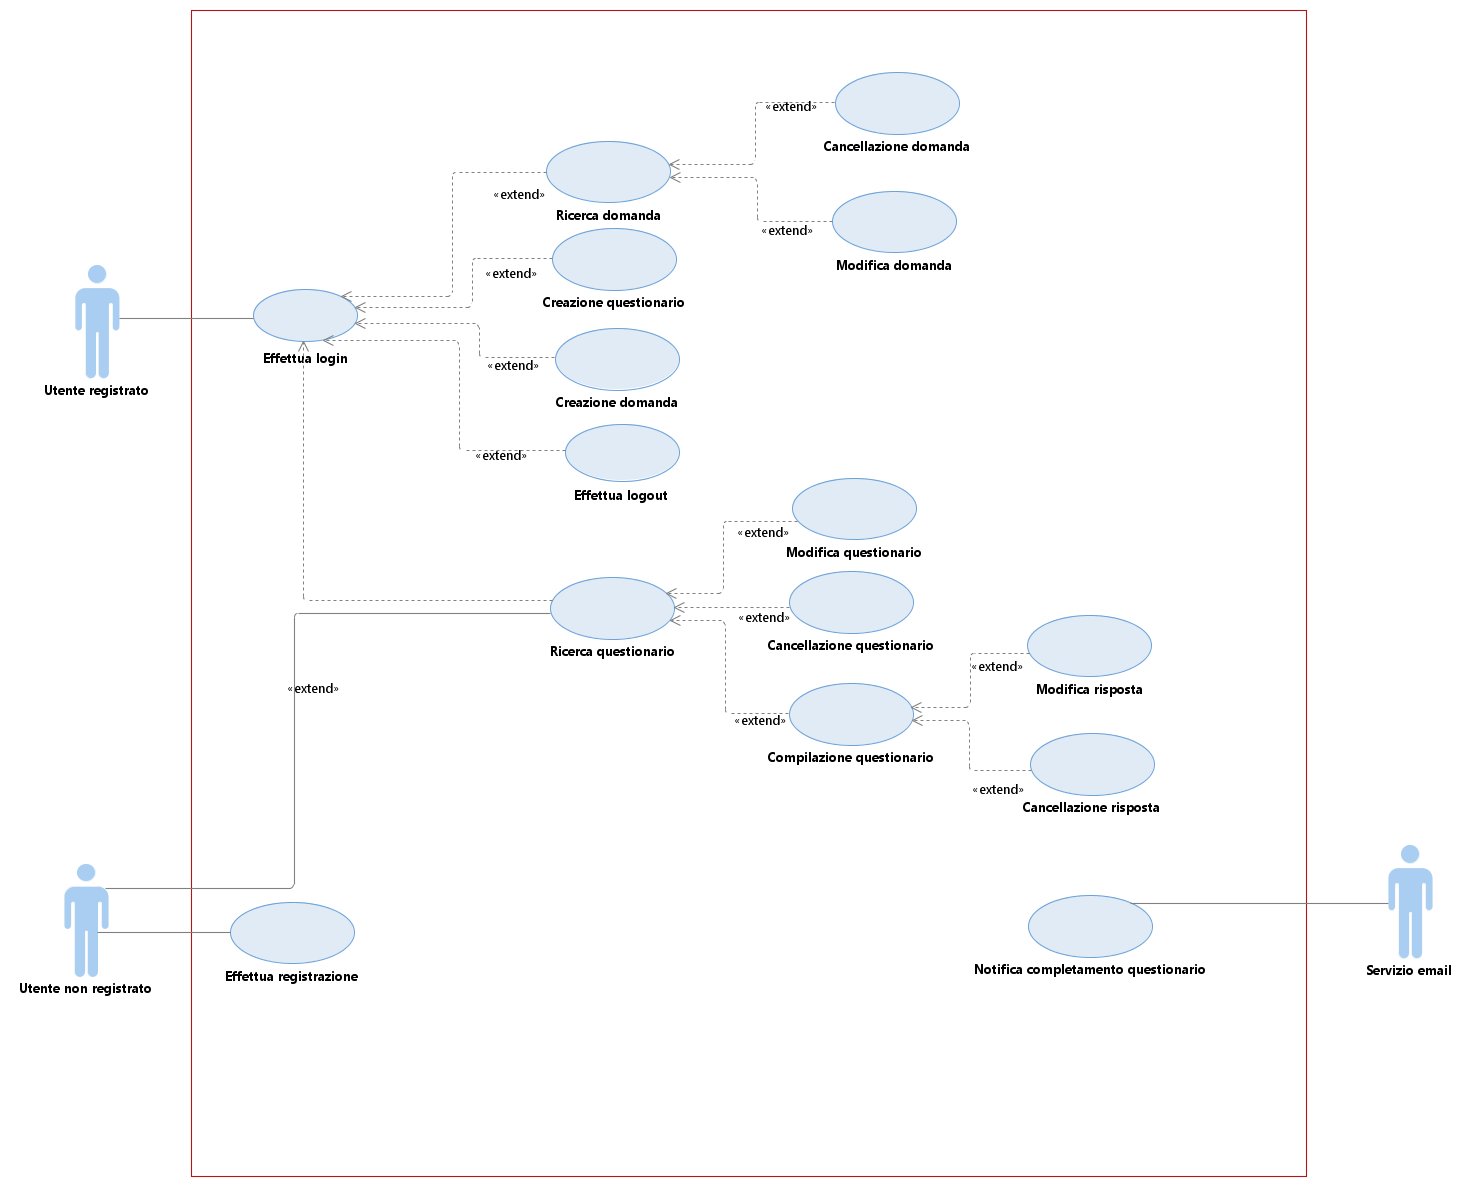
\includegraphics[scale=0.45, left]{fig_usecase_diagram.png}
\caption{Diagramma dei casi d'uso}
\end{figure}

\subsection{Requisiti non funzionali}

\begin{table}[H]
\begin{adjustbox}{max width=1.1\textwidth,center}
\begin{tabular}{|l|l|l|l|}
\hline
\rowcolor[HTML]{3531FF} 
{\color[HTML]{FFFFFF} ID} & {\color[HTML]{FFFFFF} Descrizione}                                                      & {\color[HTML]{FFFFFF} Tipo} & {\color[HTML]{FFFFFF} Misura} \\ \hline
1                         & Il sistema deve essere sempre raggiungibile                                             & Di prodotto                 & Disponibilità                 \\ \hline
2                         & Il sistema deve essere in grado di gestire molti utenti contemporaneamente              & Di prodotto                 & Efficienza                    \\ \hline
3                         & Il sistema deve garantire la persistenza dei dati                                       & Di prodotto                 & Affidabilità                  \\ \hline
4                         & Il sistema deve garantire la sicurezza dei dati degli utenti                            & Di prodotto                 & Sicurezza                     \\ \hline
5                         & Il sistema deve garantire brevissime attese agli utenti per l'elaborazione di richieste & Di prodotto                 & Efficienza                    \\ \hline
\end{tabular}
\end{adjustbox}
\end{table}





\subsection{Design Principles}
Design Principles utilizzati durante la creazione del progetto.
\begin{itemize}
	\item \textbf{Principio di sostituzione di Liskov}: Gli oggetti di un sottotipo di un oggetto possono essere sostituiti dall'oggetto di cui sono sottotipo senza alterare la correttezza del programma.
	\item \textbf{Principio di inversione delle dipendenze}: I moduli di alto e basso livello non dipendono tra di loro ma dipendono da astrazioni.
	\item \textbf{Principio di segregazione delle interfacce}: Il client utilizza interfacce piccole e specifiche ma numerose per evitare dipendenza da metodi non utilizzati.
	\item \textbf{Principio delle dipendenze acicliche}: Il grafo delle dipendenze di pacchetti non presenta cicli.
\end{itemize}

\subsection{SSD}
Qui di seguito sono presenti gli SSD riguardanti i seguenti scenari:
\begin{itemize}
\item Creazione del questionario
\end{itemize}

\begin{figure}[H]
\centering
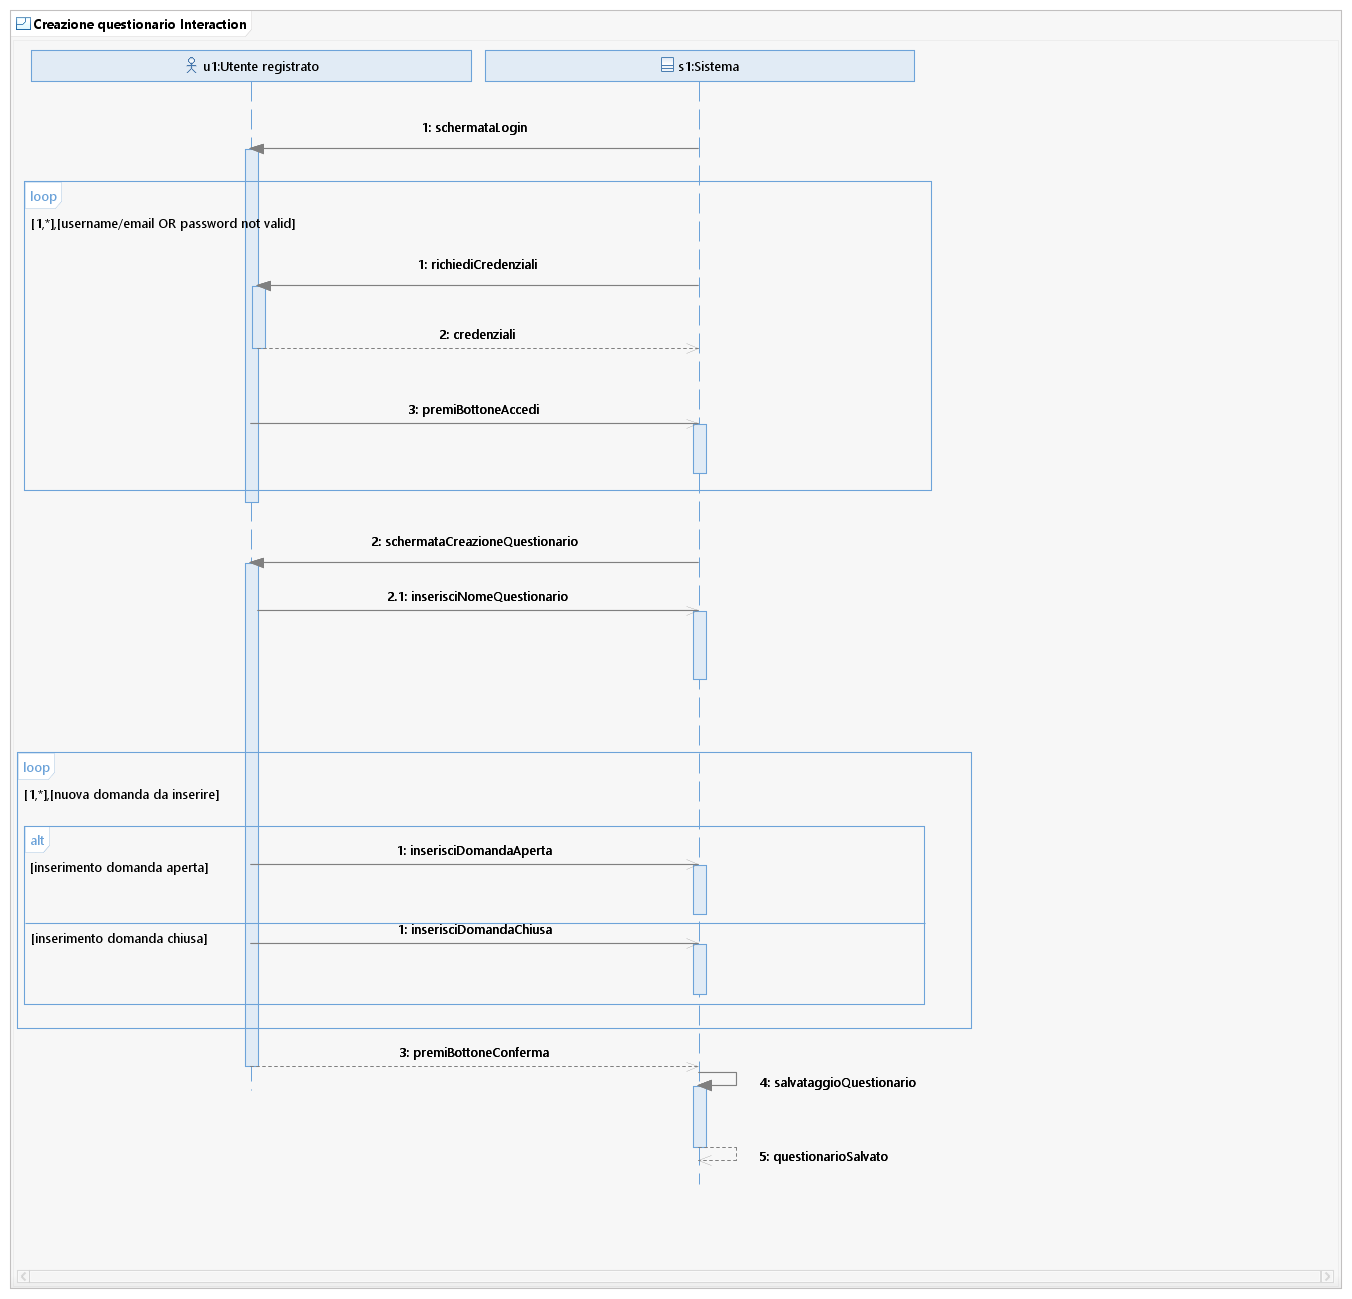
\includegraphics[scale=0.47]{UNIMIBModule_CreazionequestionarioSequenceDiagram.png}
\caption{SSD - Creazione del questionario}
\end{figure}



\subsection{Modello di dominio}
\begin{figure}[H]
\centering
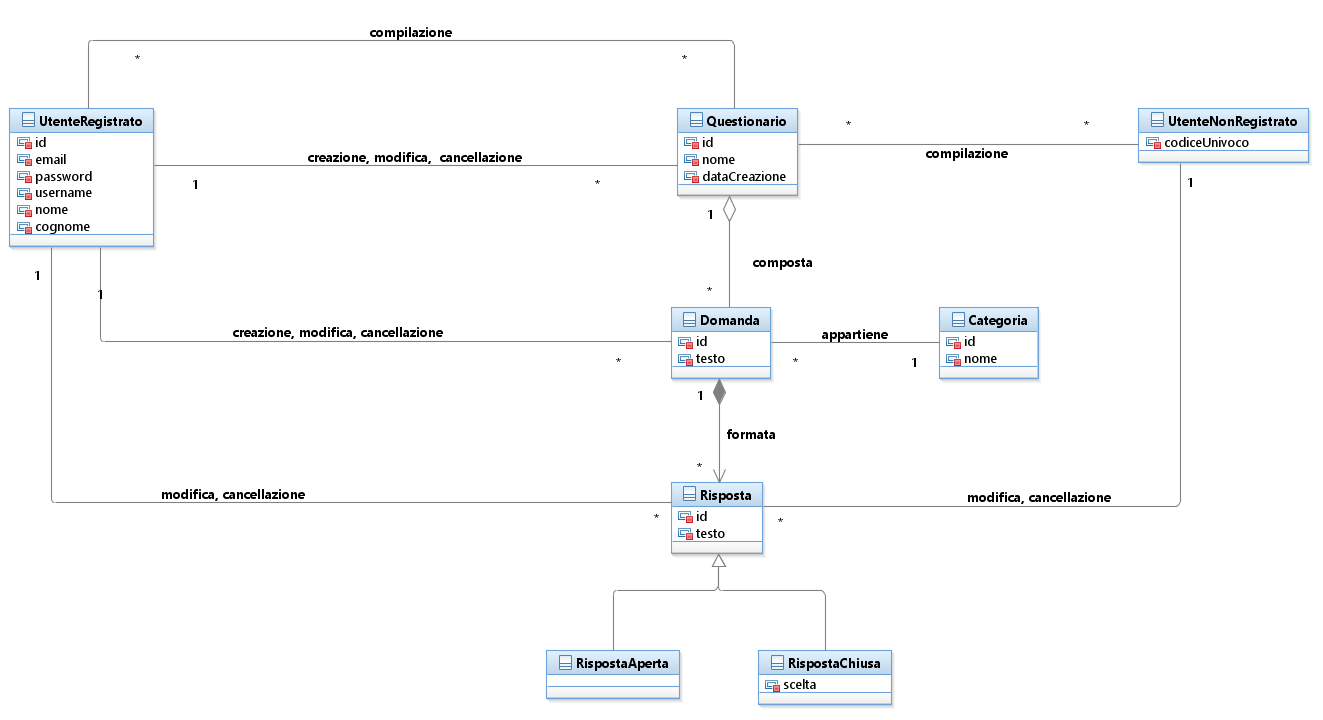
\includegraphics[scale=0.5]{UNIMIBModule_UniMiBModuleDomainLayer.png}
\caption{Modello di dominio}
\end{figure}
\subsection{Diagramma delle classi di progettazione}
\subsection{Diagrammi di sequenza}
\subsubsection{aggiugiDomanda}
\begin{figure}[H]
\centering
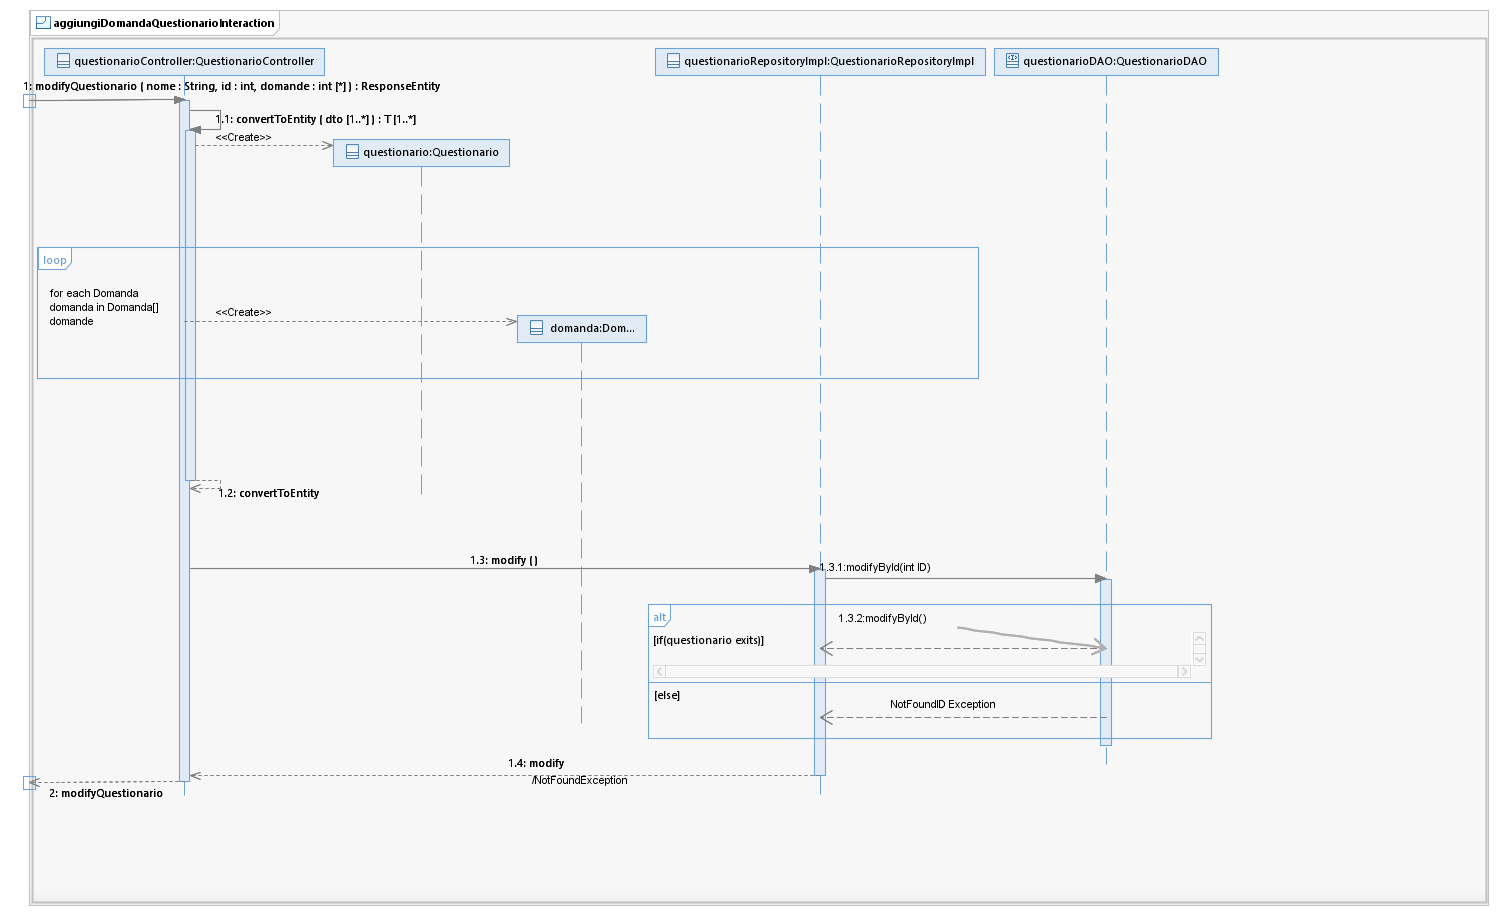
\includegraphics[scale=0.40]{UNIMIBModule_aggiungiDomandaQuestionarioSequenceDiagram.png}
\caption{Diagramma di sequenza aggiungiDomanda}
\end{figure}
\subsubsection{eliminaDomanda}
\begin{figure}[H]
\centering
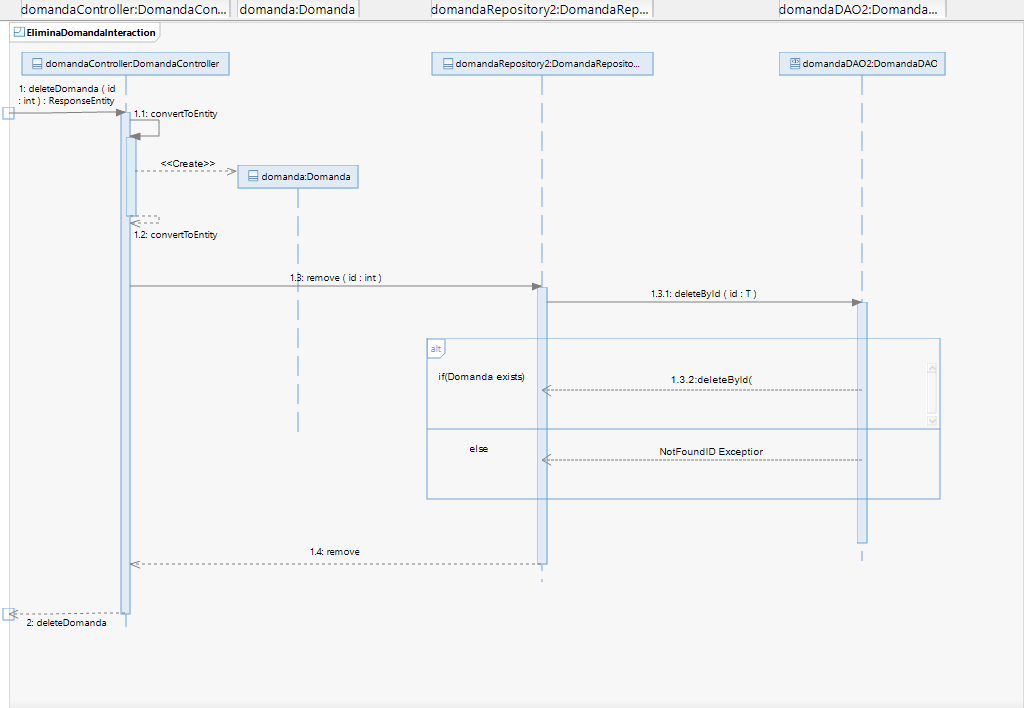
\includegraphics[scale=0.40]{UNIMIBModule_EliminaDomandaSequenceDiagram.png}
\caption{Diagramma di sequenza eliminaDomanda}
\end{figure}
\subsection{Diagrammi di stato}
\subsubsection{StateMachine Creazione Questionario}
\begin{figure}[H]
\centering
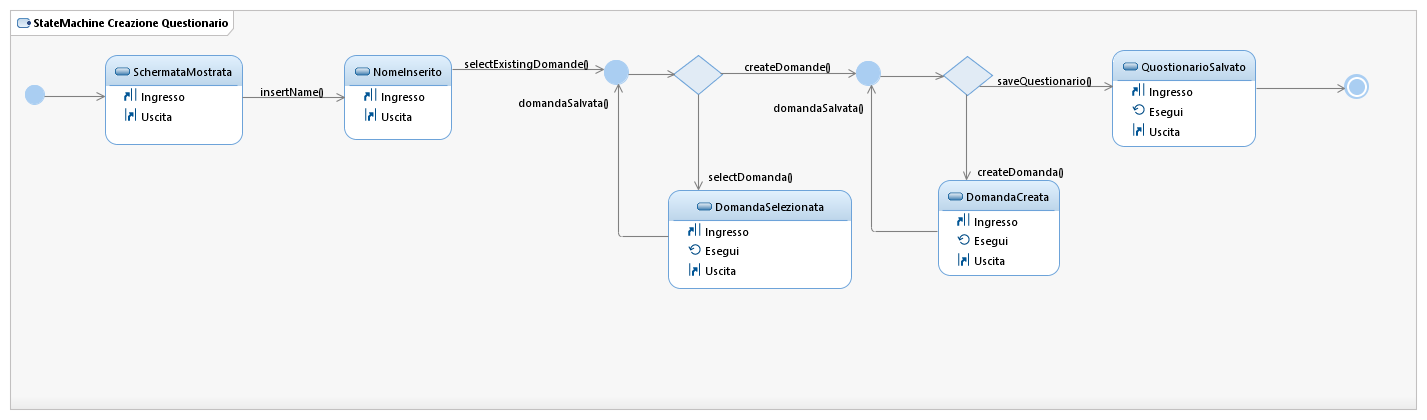
\includegraphics[scale=0.40]{UNIMIBModule_StatemachineDiagramCreazioneQuestionario.png}
\caption{Diagrammi di stato creazioneQuestionario}
\end{figure}
\subsection{Diagrammi di attivit\`{a}}
\subsubsection{Creazione Questionario}
\begin{figure}[H]
\centering
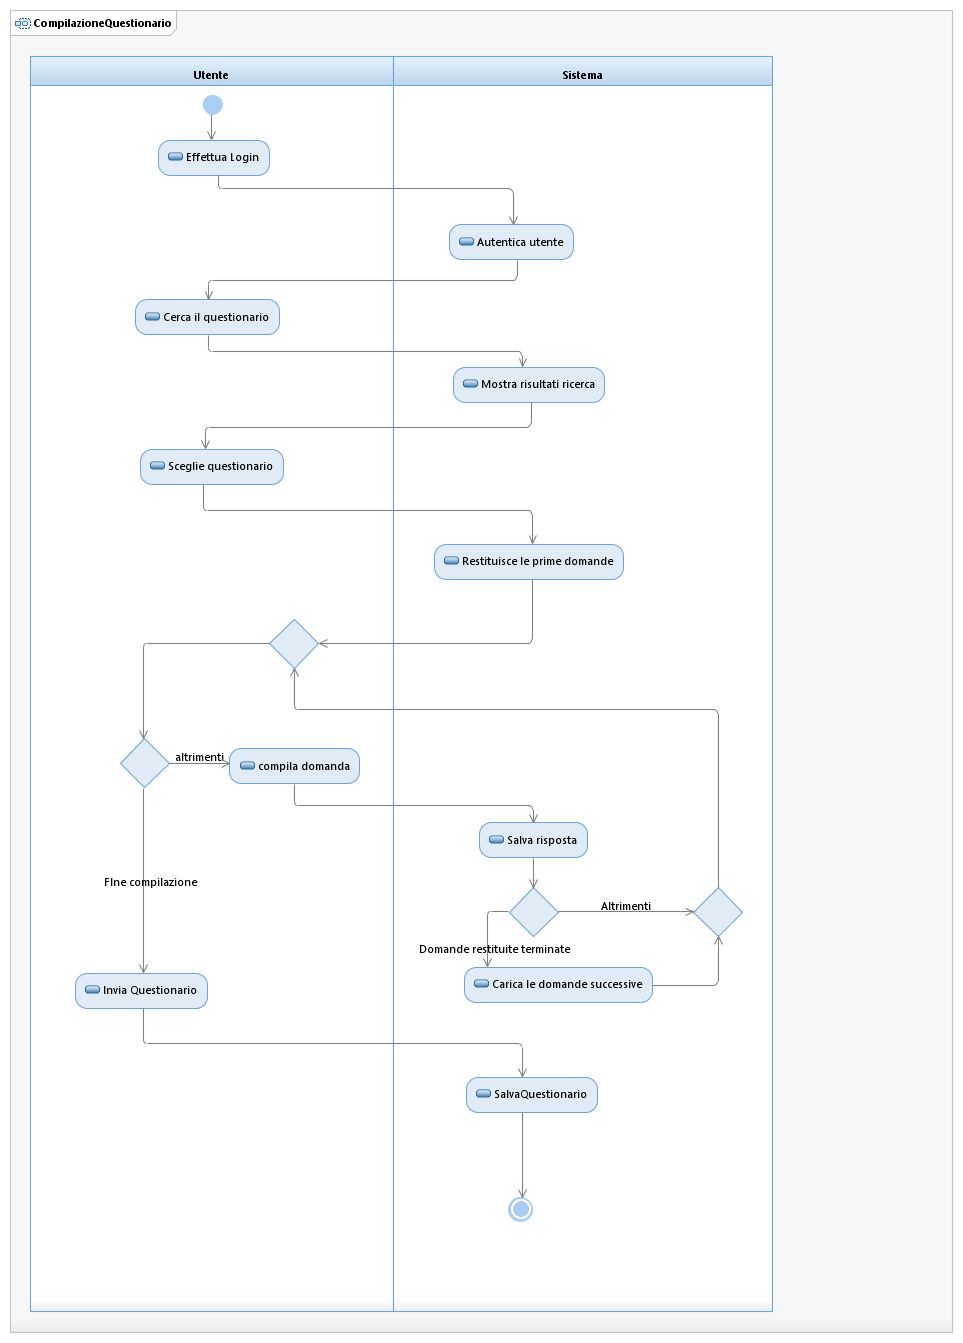
\includegraphics[scale=0.47]{UNIMIBModule_CompilazioneQuestionarioActivityDiagram.png}
\caption{Diagramma di attività creazioneQuestionario}
\end{figure}
\subsection{Diagramma dell'architettura software}
\begin{figure}[H]
\centering
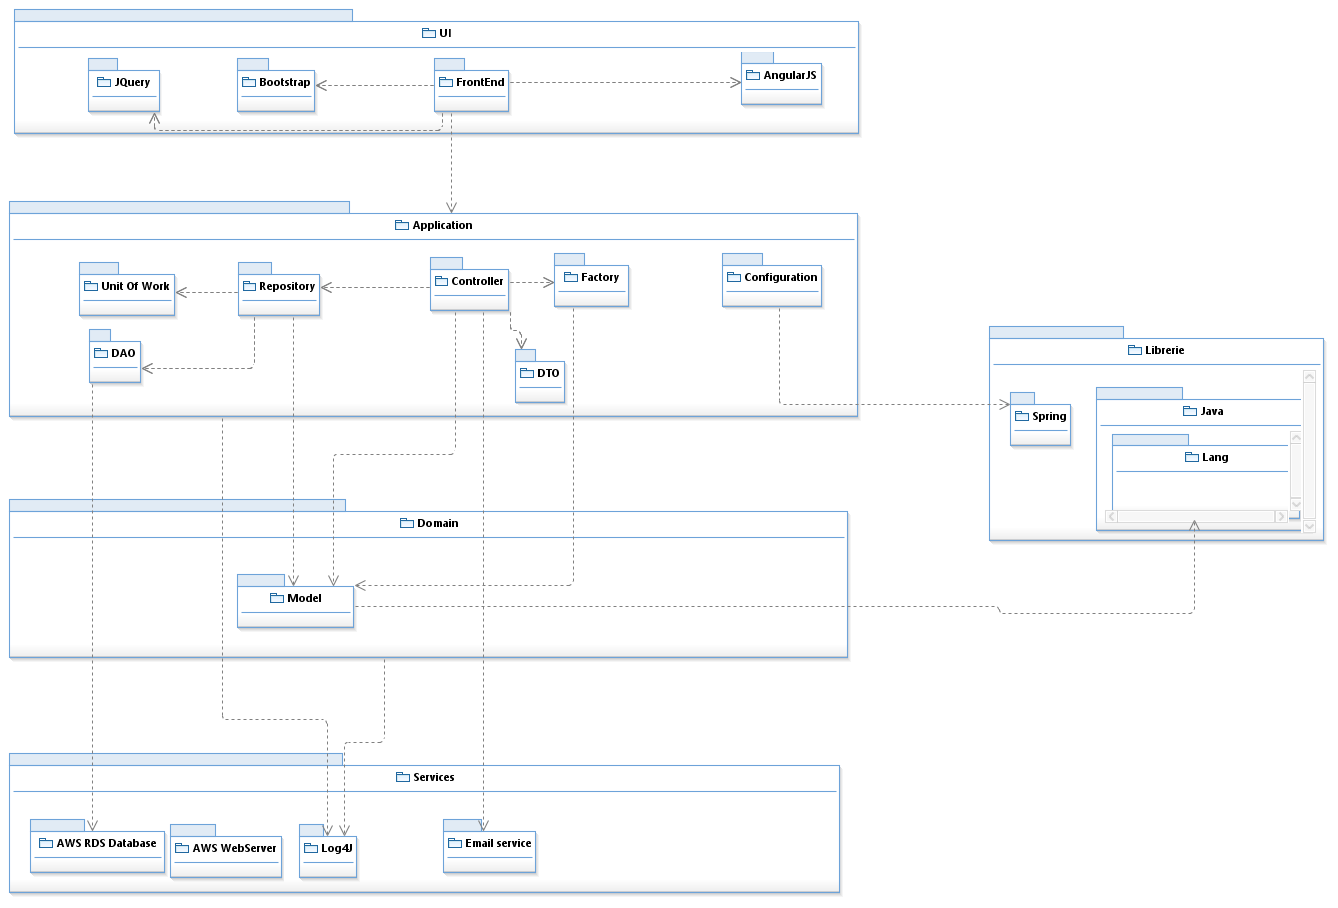
\includegraphics[scale=0.5]{UNIMIBModule_LogicalArchitectureDiagram.png}
\caption{Diagramma dell'architettura software}
\end{figure}
\subsection{Design Patterns}
Design Patterns utilizzati durante la creazione del progetto.
\subsubsection{Architectural Patterns}
	\begin{itemize}
		\item \textbf{Unit of Work}
    	\begin{itemize}
            \item \textbf{Nome}: Unit of Work
            \item \textbf{Classificazione}: Architectural
            \item \textbf{Applicabilità}: Nel caso di UnimibModules quando l'utente sta compilando un questionario, le risposte non vengono inserite/modificate/eliminate appena l'utente conferma; vengono inserite nella Unit Of Work e vengono poi salvate quando l'utente termina la compilazione.
            \item \textbf{Partecipanti}:
                \begin{itemize}
                    \item {UnitOfWork}
                    \item {RispostaRepositoryImpl}
                    
                \end{itemize}
            \item \textbf{Scopo}: Classe che si occupa di tenere traccia di ciò che possa modificare il database durante una transazione business e quando è terminata si occupa di applicare tutte le modifiche.
             \item \textbf{Codice d'esempio}
            \begin{lstlisting}
/**
* The context of the UnitOfWork
 */
private final Map<String, List<Answer>> uofContext;

/**
* Registers <code>answer</code> on the specified <code>operation</code>.
* @param	answer		the answer to be registered
* @param	operation	the operation to be performed on answer
*/
private void register(Answer answer, String operation) {

List<Answer> answerToOperate = uofContext.computeIfAbsent(operation, k -> new ArrayList<>());
answerToOperate.add(answer);
}

/**
* Adds <code>answer</code> to the elements to be inserted.
* @param	answer	the new Answer
* @see UnitOfWork#registerNew
*/
@Override
public void registerNew(Answer answer) {

logger.debug("Registering Answer with id {} for insert in context.", answer.getId());
register(answer, UnitOfWork.INSERT);
}

/**
* Adds <code>answer</code> to the elements to be modified.
* @param	answer	the answer that will replace the Answer with the same id
* @see UnitOfWork#registerModified
*/
@Override
public void registerModified(Answer answer) {

logger.debug("Registering Answer with id {} for modify in context.", answer.getId());
register(answer, UnitOfWork.MODIFY);
}
            \end{lstlisting}
        \end{itemize}
        
        
		\item \textbf{Data Mapper}
		\begin{itemize}
            \item \textbf{Nome}: Data Mapper
            \item \textbf{Classificazione}: Architectural
            \item \textbf{Applicabilità}: Nel caso di UnimibModules, si effettua il mapping per la conversione dei dati sia da un recupero dati dal database e sia per un invio dati verso il database
            \item \textbf{Partecipanti}:
                \begin{itemize}
                    \item CategoriaDAO
                    \item Categoria
                    \item RispostaDAO
                    \item Risposta
                    \item DomandaDAO
                    \item Domanda
                    \item QuestionarioDAO
                    \item Questionario
                    \item UtenteDAO
                    \item Utente
                    \item RispostaChiusaDAO
                    \item RispostaChiusa
                \end{itemize}
            \item \textbf{Scopo}: Classe che si occupa della conversione dei dati tra database e dominio
        \end{itemize}
		
		
		\item \textbf{Front Controller}: Oggetto che fornisce un punto centralizzato per la gestione delle richieste
		
		
		\item \textbf{Lazy Loading}
		\begin{itemize}
            \item \textbf{Nome}: Data Mapper
            \item \textbf{Classificazione}: Architectural
            \item \textbf{Applicabilità}: Nel caso di UnimibModules, quando si desidera caricare tutti i questionario o tutte le domande di questionario, queste non verranno mostrate tutte contemporaneamente ma si applicherà il lazy loading. Attraverso un offset si recupereranno un numero definito di domande alla volta.
            \item \textbf{Partecipanti}:
                \begin{itemize}
                    \item QuestionarioController
                    \item QuestionarioRepositoryImpl
                    \item DomandaController
                    \item DomandaRepositoryImpl
                \end{itemize}
            \item \textbf{Scopo}: Rinvia l'inizializzazione di un oggeto fino a quando non è necessario
            \item \textbf{Codice d'esempio}
            \begin{lstlisting}
/**
* Finds all surveys without their questions.
* 
* @return an HTTP response with status 200 if one survey exists at least.
* @throws NotFoundException
* @see it.unimib.unimibmodules.exception.NotFoundException
* @see it.unimib.unimibmodules.exception.ExceptionController
#handleNotFoundException
*/
@GetMapping("/findAllSurveysNoQuestionLazy")
public ResponseEntity<List<SurveyDTO>> findAllSurveysNoQuestionLazy(@RequestParam int offset, 
	@RequestParam int limit) throws NotFoundException {

Iterable<Survey> surveys = surveyRepository.getAllLazy(offset, limit);
logger.debug("Retrieved all Surveys.");
List<SurveyDTO> surveysDTO = new ArrayList<>();
for (Survey survey : surveys) {
	surveysDTO.add(convertToDTOAndSkipQuestions(survey));
}
logger.debug("Retrieved {} surveys.", surveysDTO.size());
return new ResponseEntity<>(surveysDTO, HttpStatus.OK);
}

/**
* Returns all surveys in the database with Lazy loading.
* @param offset
* @param limit
* @return a Set of Surveys
* @throws NotFoundException
* @see SurveyRepository#getAll()
*/
@Override
public Iterable<Survey> getAllLazy(int offset, int limit) throws NotFoundException {
Iterable<Survey> surveys = surveyDAO.findAllLazy(offset, limit);
if (IterableUtils.size(surveys) > 0) {
	return surveys;
} else {
	throw new NotFoundException("No surveys exist.");
}
}
            \end{lstlisting}
        \end{itemize}
	\end{itemize}
\subsubsection{Data Patterns}
	\begin{itemize}
		\item \textbf{Data Transfer Object}
		\begin{itemize}
		\item \textbf{Nome}: Data Transfer Object
            \item \textbf{Classificazione}: Data
            \item \textbf{Applicabilità}: Nel caso di UnimibModules, quando si vogliono inviare dati al client o si ricevono dati dal client, questi vengono trasportati attraverso il corrispondente DTO.
            \item \textbf{Partecipanti}:
                \begin{itemize}
                    \item DTOMapping
                    \item UtenteDTO
                    \item UtenteController
                    \item QuestionarioDTO
                    \item QuestionarioController
                    \item DomandaDTO
                    \item Domanda Controller
                    \item RispostaDTO
                    \item RispostaController
                    \item RispostaChiusaDTO
                    \item RispostaChiusaController
                    \item CategoriaDTO
                    \item QuestionarioDomandeDTO
                \end{itemize}
            \item \textbf{Scopo}: Oggetto che trasporta data tra i processi per poter ridurre il numero di chiamate ai metod
            \item \textbf{Codice d'esempio}
            \begin{lstlisting}
public abstract class DTOMapping<M, T> {

/**
 * The instance of modelMapper that will be used to convert Question to QuestionDTO and vice versa.
 */
protected final ModelMapper modelMapper;

@Autowired
protected DTOMapping(ModelMapper modelMapper) {

	this.modelMapper = modelMapper;
	modelMapper.getConfiguration().
	setMatchingStrategy(MatchingStrategies.STANDARD);
	modelMapper.getConfiguration().setImplicitMappingEnabled(false);
}

/**
 * Converts an instance of M to an instance of T
 * @param	value	an instance of M
 * @return			an instance of T, containing the serialized data of value
 */
public abstract T convertToDTO(M value);

/**
 * Converts an instance of T to an instance of M
 * @param   dto	an instance of T
 * @return		an instance of M, containing the deserialized data of T
 * @throws	FormatException
 * @throws	EmptyFieldException	when one of the required field is empty
 * @throws	NotFoundException	when one of the queries fails
 * @throws	IncorrectSizeException
 */
public abstract M convertToEntity(T dto) throws FormatException, EmptyFieldException, NotFoundException, IncorrectSizeException;
}

public class QuestionDTO {

	/**
	 * Serialization of the id of the question.
	 */
	@Getter	private int id;

	/**
	 * Serialization of the category of the question.
	 */
	@Getter	@Setter private CategoryDTO category;
	
	/**
	 * Serialization of the image's url of the question.
	 */
	@Getter	@Setter private String urlImage;
	
	/**
	 * Serialization of the text of the question.
	 */
	@Getter	@Setter private String text;

	/**
	 * Modifies the id of the question, setting <code>id</code> as the new value.
	 * @param	id	the new id value
	 */
	public void setId(int id) {

		this.id = id;
	}

	/**
	 * Modifies the id of the question, setting <code>id</code> as the new value.
	 * @param	id	the new id value
	 */
	public void setId(Object id) {

		this.id = (int) id;
	}
}

public class QuestionController extends DTOListMapping<Question, QuestionDTO>{

public QuestionController(QuestionRepository questionRepository) {

super(modelMapper);

modelMapper.createTypeMap(Question.class, QuestionDTO.class)
		.addMappings(mapper -> {
			mapper.map(Question::getId, QuestionDTO::setId);
			mapper.map(Question::getUrlImage, QuestionDTO::setUrlImage);
			mapper.map(Question::getText, QuestionDTO::setText);
			mapper.map(Question::getCategory, QuestionDTO::setCategory);
		});

modelMapper.createTypeMap(QuestionDTO.class, Question.class)
		.addMappings(mapper -> {
			mapper.map(QuestionDTO::getId, Question::setId);
			mapper.map(QuestionDTO::getUrlImage, Question::setUrlImage);
			mapper.map(QuestionDTO::getText, Question::setText);
			mapper.map(QuestionDTO::getQuestionType, Question::setQuestionType);
		});
}
            \end{lstlisting}
		\end{itemize}
		
		\item \textbf{Data Access Object}
		\begin{itemize}
		\item \textbf{Nome}: Data Access Object
            \item \textbf{Classificazione}: Data
            \item \textbf{Applicabilità}: Nel caso di UnimibModules, quando si vogliono effettuare operazioni su entità di una o più tabelle, lo si può fare attraverso i DAO, dove oltre le operazioni base sono state aggiunte in alcuni casi operazioni custom per interagire con il database.
            \item \textbf{Partecipanti}:
                \begin{itemize}
                    \item CategoriaDAO
                    \item CategoriaRepositoryImpl
                    \item RispostaDAO
                    \item RispostaRepositoryImpl
                    \item DomandaDAO
                    \item DomandaRepositoryImpl
                    \item QuestionarioDAO
                    \item QuestionarioRepositoryImpl
                    \item UtenteDAO
                    \item UtenteRepositoryImpl
                    \item RispostaChiusaDAO
                    \item RispostaChiusaRepositoryImpl
                \end{itemize}
            \item \textbf{Scopo}: Oggetto che rappresenta un'entità di una tabella di un database usato per stratificare e isolare l'accesso ad una tabella
            \item \textbf{Codice d'esempio}
            \begin{lstlisting}
public interface AnswerDAO extends CrudRepository<Answer, Integer> {

@Query("SELECT a FROM Answer a WHERE a.survey.id = :surveyId AND a.user.id = :userId")
Iterable<Answer> findSurveyAnswersForUser(@Param("surveyId") int surveyId, @Param("userId") int userId);
}

public class AnswerRepositoryImpl implements AnswerRepository, UnitOfWork<Answer>  {

/**
 * The instance of AnswerDAO that will be used to perform actions to the DB
 */
private final AnswerDAO answerDAO;

public Iterable<Answer> getSurveyAnswersForUser(int surveyId, int userId) {

return answerDAO.findSurveyAnswersForUser(surveyId, userId);
    }
}
            \end{lstlisting}
        \end{itemize}
		
		\item \textbf{Repository}
		\begin{itemize}
		\item \textbf{Nome}: Repository
            \item \textbf{Classificazione}: Data
            \item \textbf{Applicabilità}: Nel caso di UnimibModules, le interfacce Repository permettono di fare da intermediario tra l'accesso ai dati che sia controller o DAO con il resto dell'applicazione
            \item \textbf{Partecipanti}:
                \begin{itemize}
                    \item RispostaRepository
                    \item RispostaController
                    \item UtenteRepository
                    \item UtenteController
                    \item DomandaRepository
                    \item DomandaController
                    \item QuestionarioRepository
                    \item QuestionarioController
                \end{itemize}
            \item \textbf{Scopo}: Interfaccia che si occupa di mediare tra la logica di accesso dati e il resto dell'applicazione
            \item \textbf{Codice d'esempio}
            \begin{lstlisting}
public interface CategoryRepository {

/**
 * Finds the category identified by id in the database
 * @param   id  the id of the category to be found
 * @return      an instance of Category if there is a category identified by id, null otherwise
 */
Category get(int id) throws NotFoundException;

/**
 * Finds all the categories in the database
 * @return      all the instances of Category, null otherwise
 */
Iterable<Category> getAll() throws NotFoundException;
}

public class CategoryController extends DTOListMapping<Category, CategoryDTO>{

    /**
     * Instance of CategoryRepository that will be used to access the db.
     */
    private final CategoryRepository categoryRepository;


    @Autowired
    public CategoryController(CategoryRepository categoryRepository) {

        super(modelMapper);
        this.categoryRepository = categoryRepository;
    }

    /**
     * Gets the Category associated with the given id.
     * @param	id	the id of the category
     * @return		an HTTP response with status 200, 500 otherwise
     * @throws NotFoundException 
     */
    @GetMapping(path = "/findCategory/{id}")
    public ResponseEntity<CategoryDTO> findCategory(@PathVariable int id) throws NotFoundException {
        Category category = categoryRepository.get(id);
        return new ResponseEntity<>(convertToDTO(category), HttpStatus.OK);
    }
}
            \end{lstlisting}
        \end{itemize}
		
		
		\item \textbf{Abstract factory}
		\begin{itemize}
		\item \textbf{Nome}: Abstract Factory
            \item \textbf{Classificazione}: Data
            \item \textbf{Applicabilità}: Nel caso di UnimibModules, le interfacce Factory permettono la creazione degli oggetti delle classi principali nel dominio.
            \item \textbf{Partecipanti}:
                \begin{itemize}
                    \item RispostaFactory
                    \item Risposta
                    \item DomandaFactory
                    \item Domanda
                    \item QuestionarioFactory
                    \item Questionario
                    \item UtenteFactory
                    \item Utente
                \end{itemize}
            \item \textbf{Scopo}: Interfaccia che permette di creare famiglie di oggetti connessi o dipendenti tra loro
            \item \textbf{Codice d'esempio}
            \begin{lstlisting}
public class AnswerFactory {

private AnswerFactory() {

    throw new IllegalStateException("Utility class");
}

/**
* Creates a new instance of Answer.
* @param	text				the text of the answer
* @param	user				the instance of the user who created the answer
* @param	survey				the instance of the survey related to this answer
* @param	question			the instance of the question related to this answer
* @return						the newly created instance of Answer
* @throws	EmptyFieldException	if the answer is empty
*/
public static Answer createAnswerToOpenQuestion(String text, User user, Survey survey, Question question)
    throws EmptyFieldException {
    
    Answer answer = new Answer();
    answer.setUser(user);
    answer.setSurvey(survey);
    answer.setQuestion(question);
    answer.setText(text);
    return answer;
    }
}
            \end{lstlisting}
        \end{itemize}
		
		
		\item \textbf{Façade}
		\begin{itemize}
		\item \textbf{Nome}: Façade
            \item \textbf{Classificazione}: Data
            \item \textbf{Applicabilità}: Nel caso di UnimibModules, Façade permette l'accesso ai vari controller Spring
            \item \textbf{Scopo}: Rappresenta il sistema complessivo, un oggetto radice, un dispositivo all’interno del quale viene eseguito il software, un punto di accesso al software o un sottosistema principale.
        \end{itemize}
	\end{itemize}
	
\subsubsection{Security Patterns}
	\begin{itemize}
		\item \textbf{Valet Key}
    	\begin{itemize}
            \item \textbf{Nome}: Valet Key
            \item \textbf{Classificazione}: Security
            \item \textbf{Applicabilità}: Nel caso di UnimibModules, ogni domanda può contenere un'immagine e, per motivi di performance, è stato affidato al dispositivo client il compito di ottenere o inviare le immagini al service storage. Il valtet key si occupa della sicurezza durante l'interazione tra il client e il data storage.
            \item \textbf{Partecipanti}: DA SISTEMARE + LINK SEZIONE AWS
                \begin{itemize}
                    \item {AWSToken}
                    \item {AWSTokenImpl}
                    \item {QuestionController}
                \end{itemize}
            \item \textbf{Scopo}: Gestire l'accesso a risorse protette da parte degli endpoint client, autenticati nel sistema, fornendogli il valet key.
             \item \textbf{Codice d'esempio} METTIAMO LE CLASSI AWSTOKEN ED UN ESEMPIO CLIENT TIPO LA GET
             
             \end{itemize}
             \end{itemize}
             
\subsection{Architettura di deployment}
\subsubsection{Diagramma di deployment}
\subsubsection{AWS - Amazon Web Services}
\begin{figure}[H]

\includegraphics[scale=0.08, left]{aws-logo.png}
\end{figure}
L'intera infrastruttura dell'applicazione si basa sui servizi offerti da AWS (Amazon Web Services). AWS offre servizi di cloud computing, on-demand e pay-per-use, che possono appartenere alle classi IAAS (es. EC2, Load balancer), PAAS (es. Cloud9, Elastic Beanstalk) e SAAS (es. SNS). L'applicazione è raggiungibile al segue link: \textcolor{blue}{\href{http://unimibquestionari-env.eba-3behr9mi.eu-central-1.elasticbeanstalk.com/}{UnimibModules}}. In questa sezione dell'analisi sono descritti i servizi utilizzati in UnimibModules. 
\begin{itemize}
\item \textbf{RDS - Relational Database Service}
\begin{figure}[H]

\includegraphics[scale=0.1, left]{rds.png}
\end{figure}
RDS è stato utilizzato come database dell'applicazione. Inoltre, per poter garantire la persistenza dei dati è stato attivato il backup automatico. Un estensione dell'utilizzo attuale consiste nell'abilitazione dei replica sets per poter garantire ancora più affidabilità al sistema.
\item \textbf{Elastic Beanstalk}
\begin{figure}[H]

\includegraphics[scale=0.3, left]{elastic.png}
\end{figure}
Elastic Beanstalk si trova al centro dell'intera infrastruttura dell'applicazione. Esso è un servizio PAAS che facilita la distribuzione di applicazioni web andando ad astrarre la gestione delle istanze fisiche EC2 e il processo stesso di installazione e distribuzione delle versioni applicative. Nel caso di UnimibModules il servizio dispone  un ambiente Java con auto scaling e load balancing. Il load balancing permette di distribuire le richieste su diverse istanze EC2 garantendo la disponibilità  e tolleranza del sistema ad eventuali fault delle macchine fisiche. L'auto scaling interagisce con il load balancing andando ad aggiungere o rimuovere elementi dal pool di istanze EC2 per poter minimizzare l'utilizzo di forza computazionale nei momenti di basso carico  e per poter rispondere al meglio nelle situazioni di carico opposte.
\item \textbf{S3 - Simple Storage Service}
\begin{figure}[H]

\includegraphics[scale=0.2, left]{s3.png}
\end{figure}
S3 è un servizio che permette l'archiviazione di oggetti all'interno di buckets. Gli oggetti possono essere di qualsiasi tipo, ma nel caso di UnimibModules si tratta solamente di immagini riferite alle domande del sistema. S3 garantisce sicurezza negli accessi, disponibilità e persistenza dei dati tramite i backup automatici. Utilizzando questo servizio non è più necessario archiviare le immagini direttamente nel file system dell'istanza che esegue l'applicazione, ma si dividono le entità per migliorare in generale le performance applicative. Il bucket UnimibModules non è pubblico, quindi è protetto da policy di sicurezza AWS.
\item \textbf{IAM - Identity and Access Management}
\begin{figure}[H]

\includegraphics[scale=0.2, left]{iam.png}
\end{figure}
Nell'applicazione UnimibModules, IAM è stato utilizzato per poter creare la policy di accesso ad S3, sfruttata dal role associato all'identity pool di Cognito. La policy concede l'accesso al bucket S3 per le operaazioni di PUT, GET e DELETE.
\item \textbf{Cognito}
\begin{figure}[H]

\includegraphics[scale=0.2, left]{cognito.png}
\end{figure}
Cognito permette di aggiungere strumenti di registrazione degli utenti, accesso e controllo degli accessi alle app Web e per dispositivi mobili. Tutto questo integrandosi con vari identity provider come google, facebook o costum. Un'altra sua applicazione riguarda la gestione degli accessi da parte degli utenti e risorse remote. Questo ultimo caso riguarda proprio il campo di utilizzo del servizio in UnimibModules. Per permettere agli utenti di comunicare direttamente con il bucket S3, per poter applicare il valet key, è necessario utilizzare Cognito come access manager. Si definisce quindi la differenza tra user-pool e identity-pool. Il primo è una directory che permette il login e signup degli utenti, come descritto precedentemente. Il secondo è utilizzato per gestire gli accessi  degli user  ai servizi AWS, appartenenti all'applicazione stessa, con credenziali temporanee. L'identity pool, identificato dall'identityPoolID, possiede un IAM role a cui è stata associata la policy precedentemente descritta. Questo ruolo rappresenta una matrice dalla quale andare a generare nuovi utenti temporanei. Per poter ottenere l'accesso diretto a un servizio è necessario eseguire il seguente work-flow:
\begin{itemize}
\item \textbf{1.} Autenticazione dello user con il server
\item \textbf{2.} Server: Comunicazione dell'avvenuto logging dello user a Cognito per ottenere l'identity ID e il token di accesso OpenID settandone la durata.
\item \textbf{3.} Per ottenere le vere e proprie credenziali lo user scambia il token ricevuto(token openID e identityID) con Cognito.
\item \textbf{4.} Le credenziali sono utilizzate per accedere direttamente ai servizi AWS secondo i termini della policy dell'Identity pool. 
\end{itemize}
\begin{figure}[H]
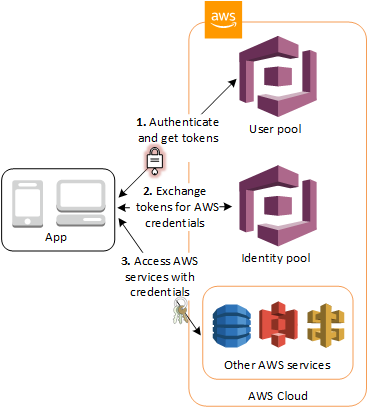
\includegraphics[scale=0.7, center]{idus.png}
\caption{Utilizzo combinato di user e identity pool}
\end{figure}
\item \textbf{STS - Security Token Service}
\begin{figure}[H]

\includegraphics[scale=0.5, left]{sts.png}
\end{figure}
STS viene utilizzato per l'effettiva generazione di chiavi di accesso temporanee a servizi AWS. Nel caso specifico viene sfruttato da Cognito per la creazione delle credenziali temporanee di S3.

\end{itemize}
\subsubsection{Valet Key - Gestione immagini}
Il Valet Key, introdotto nel capitolo dei pattern architetturali, è strettamente legato ai servizi AWS appena elencati.
\begin{figure}[H]
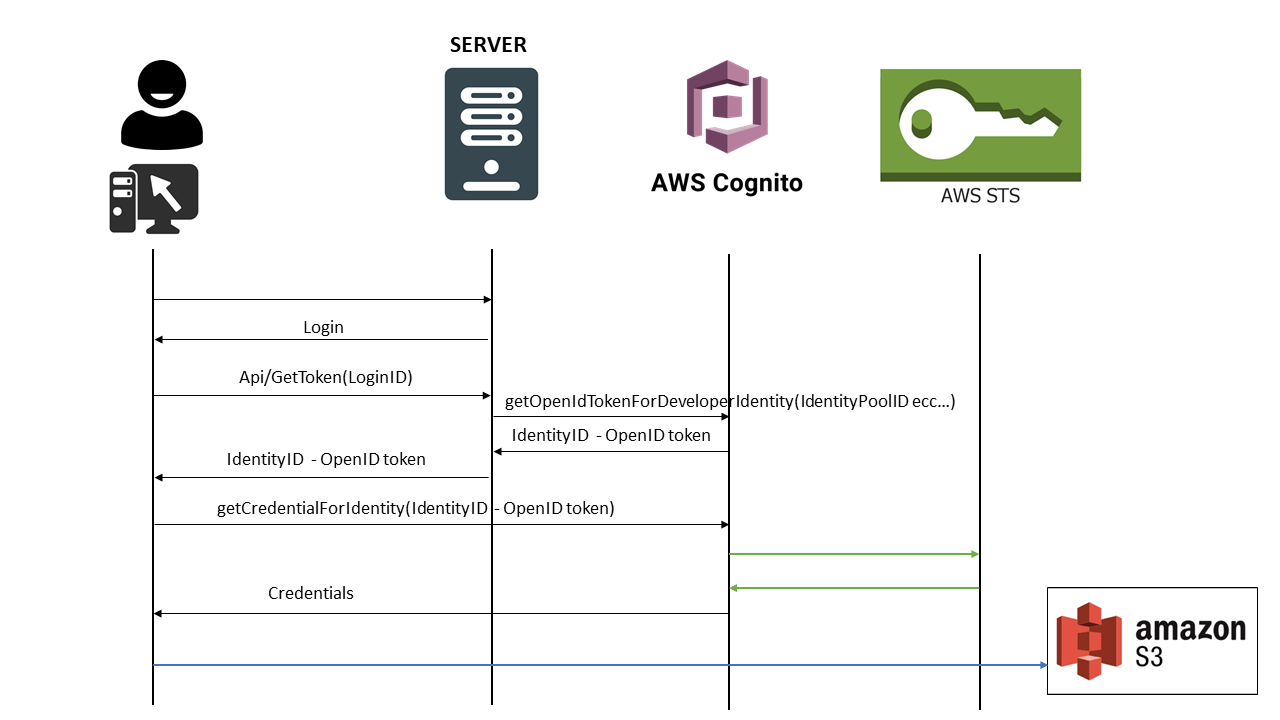
\includegraphics[scale=0.5, left]{diapAWS.png}
\caption{Valet Key- Flusso operativo}
\end{figure}
Il pattern è stato scelto per deresponsabilizzare l'applicazione dal compito di gestire gli stream di dati (upload e download) inerenti alle immagini andando a mantenere la completa sicurezza dello storage remoto, cioè S3.\\
Viene definito il seguente flusso operativo:
\begin{itemize}
\item Login - Lo user deve essere loggato nell'applicazione per poter richiedere il valet key;
\item Quando il codice client necessita, per esempio, di caricare un'immagine allegata ad una nuova domanda invia la prima richiesta all'API dell'applicazione chiamata GetToken, allegando l'ID utente per dimostrare l'effettivo passaggio dal punto precedente;
\item Il server elabora la richiesta ed esegue la chiamata al metodo getOpenIdTokenForDeveloperIdentity tramite l'AWS SDK. Il server possiede le credenziali root dell'intero sistema quindi è in grado di avviare quest'ultima funzione passando come parametri l'ID dell'identity pool a cui si fa riferimento, la regione AWS di appartenenza e la durata del token.
\item Il client ottiene dal server l'identityID (identifica un'istanza di un ruolo Cognito creato in AWS) e il token di accesso.
\item Il client esegue la richiesta delle effettive credenziali temporanee direttamente a Cognito.
\item Cognito delega il compito della creazione delle credenziali con policy pre-generata ad AWS STS.
\item Il client utilizza le credenziali per interagire con il bucket S3.
\end{itemize}

\subsection{Modello E-R}
\section{Sviluppo}
\subsection{Piano dello sprint}
\`{E} stato adottato un metodo di processo di sviluppo Agile seguendo le direttive dell' Unified Process. Il Product backlog contiene i task, normalmente associati ad un caso d'uso,  da sviluppare nei vari sprint. Ogni sprint prevede le seguenti fasi:
\begin{itemize}
\item {\textbf {Sprint meeting}} per la composizione dello sprint backlog;
\item {\textbf {Analisi e progettazione}}  per aggiornare o creare componenti UML utili al task;
\item {\textbf {Bulding e testing}}  per lo sviluppo e testing del task;
\item {\textbf {Review e refactoring}} per la revisione generale del lavoro effettuato e della qualità del codice (architectural smell, code smell ecc...);
\item {\textbf {Retrospective meeting}} per chiudere con il team lo sprint presentando problemi, modifiche ecc...
\end{itemize}
\subsection{Linguaggi}
L'applicazione web è interamente basata sul framework Java Spring. Per quanto riguarda il codice client è stato utilizzato AngularJs come middleware tra il DOM HTML e il server.
\subsection{Workflow per la Continuos Integration}


%----------------------------------------------------------------------------------------


\end{document}